
\begin{question}
In a very large pile of toothpicks, the mean length is 65.72 millimeters
and the standard deviation is 3.84 millimeters. If you randomly sample
169 toothpicks, what is the chance the sample mean is between 64.96 and
65.89 millimeters?
\end{question}

\begin{solution}
Label the given information. \[ 
\begin{aligned}
\mu &= 65.72\\
\sigma &= 3.84\\
n &= 169\\
\bar{x}_\text{lower} &= 64.96 \\
\bar{x}_\text{upper} &= 65.89
\end{aligned}
\] Find the standard error.
\[SE = \frac{\sigma}{\sqrt{n}} = \frac{3.84}{\sqrt{169}} = 0.295 \]
Describe the sampling distribution.
\[\bar{X} \sim \mathcal{N}(65.72,\,0.295) \]

Draw a sketch.\\
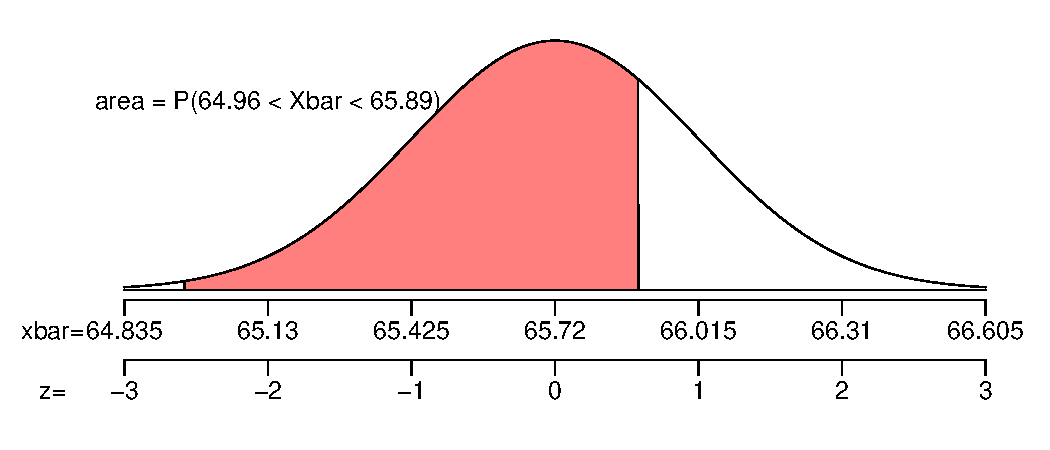
\includegraphics{normal_sketch_sampling-1.pdf} ~

Calculate a \(z\) scores.
\[z_\text{lower} = \frac{x_\text{lower}-\mu}{SE} = \frac{64.96-65.72}{0.295} = -2.58 \]
\[z_\text{upper} = \frac{x_\text{upper}-\mu}{SE} = \frac{65.89-65.72}{0.295} = 0.58 \]
Determine the probability. \[
\begin{aligned}
P(64.96 < X < 65.89) &= \Phi(z_\text{upper}) - \Phi(z_\text{lower}) \\
&= \Phi(0.58) - \Phi(-2.58) \\
&= 0.7141 
\end{aligned}
\]
\end{solution}

